\documentclass{article}
\usepackage[letterpaper,margin=0.42in,top=0.42in,bottom=0.42in]{geometry}
\usepackage{amsmath,booktabs,enumitem,graphicx,microtype,multicol,tabularx,xcolor}
\usepackage[hidelinks]{hyperref}
\usepackage{fancyhdr}
\setlength{\parindent}{0pt}
\setlength{\parskip}{1.5pt}
\setlength{\columnsep}{0.18in}
\setlist[itemize]{leftmargin=*,nosep}
\definecolor{navy}{HTML}{102A43}
\definecolor{teal}{HTML}{0B7A75}
\definecolor{amber}{HTML}{D97706}
\definecolor{pale}{HTML}{EEF6F7}
\definecolor{ink}{HTML}{243B53}
\pagestyle{fancy}
\fancyhf{}
\lhead{\scriptsize Whose Human Are You? --- Member A research brief}
\rhead{\scriptsize 15 November 2026}
\cfoot{\scriptsize \thepage\ / 2}
\renewcommand{\headrulewidth}{0.3pt}
\makeatletter
\renewcommand\section{\@startsection{section}{1}{\z@}{0.8ex plus .2ex}{0.35ex}{\normalfont\normalsize\bfseries\color{navy}}}
\makeatother
\newcommand{\status}[1]{\textcolor{teal}{\textbf{#1}}}
\newcommand{\simulated}{\textcolor{amber}{\textbf{SIMULATED --- NOT AN OBSERVED EXPERIMENT}}}
\newcommand{\term}[1]{\texttt{#1}}

\begin{document}
\fontsize{8}{9.15}\selectfont
\begin{center}
{\LARGE\bfseries\color{navy} Member A: Local-Agent Measurement and Same-PC Linking}\\[-1pt]
{\small A two-page engineering research brief for the consent-based ``Whose Human Are You?'' study}
\end{center}

\vspace{-2mm}
\colorbox{pale}{\parbox{0.965\linewidth}{\textbf{Abstract.}
Member A implemented controlled agent runs, visible text submission, an interpretable transport/runtime signature,
and a privacy-minimised local-model timing pipeline. The narrow new question is: \emph{did Omen and Queen probably
run on the same enrolled PC?} The system does not equate a PC with a human. It emits a probability-like score and
returns \term{unknown} below a high validation-selected threshold. The engineering path is implemented and tested;
no labelled multi-PC campaign has yet validated the scientific claim.}}

\begin{multicols}{2}
\section*{1. Member A implementation}
\textbf{Track 1a --- agent runs.} A manifest-safe CLI creates unique \term{a-*} run IDs, records agent, model,
pseudonymous machine, and network category, and prints one fixed task. Locality is reported only as \term{local},
\term{remote}, \term{mixed}, or \term{inconclusive}.

\textbf{Track 2a --- visible text.} Two partner sites expose article text plus visible POST and GET submission
paths. The corpus tool distinguishes successful submission, fetch without submission, unrelated traffic, and no
observed request. No hidden prompt or third-party site is used.

\textbf{Track 3b --- two evidence layers.} The server-side baseline hashes selected TLS, HTTP-runtime, header, and
HTTP/2 features:
\[
E(r)=\texttt{env-v1}:\operatorname{Trunc}_{96}
\left(\operatorname{SHA256}(\operatorname{canon}(x_r))\right).
\]
It excludes IP, cookies, site, path, timing, body, and submitted text. This identifies an observable software stack,
not CPU or GPU.

For consenting local-model experiments, a loopback-only Ollama collector runs five fixed synthetic cases. It
discards prompts and generated text, retaining approximate first-chunk time, model-reported load and evaluation
durations, counts, throughput, and chunk-interval statistics. For profile feature $x_k$,
\[
d_k(a,b)=\frac{|x_{a,k}-x_{b,k}|}{|x_{a,k}|+|x_{b,k}|+\epsilon}.
\]
A regularized logistic model estimates $p=\sigma(\beta_0+\sum_k\beta_kd_k)$. Only $p\geq\theta$ becomes
\term{probably\_same\_pc}; every lower score remains \term{unknown}.

\section*{2. Evaluation calculations}
The fixed plan has five cases and five repetitions, hence
\[
N_{\mathrm{session}}=5\times5=25\ \text{measurements}.
\]
For $m$ machines with one Omen and one Queen profile, the positive cross-agent pairs are $m$ and the possible
negative pairs are $m(m-1)$. Training caps the negative-to-positive ratio at $3{:}1$ to prevent class imbalance.

Let TP, FP, FN, and TN refer to same-PC decisions. Report
\[
P=\frac{TP}{TP+FP},\quad R=\frac{TP}{TP+FN},\quad
F_1=\frac{2PR}{P+R},
\]
plus ROC-AUC and Brier score $n^{-1}\sum_i(p_i-y_i)^2$. Entire machines, not requests, are held out. At least six
labelled PCs are required by the implementation; more are needed for a credible result.

\section*{3. Why this design?}
\begin{itemize}
\item \textbf{No JavaScript assumption:} CLI fetchers may never execute browser fingerprint code.
\item \textbf{No fake hardware telemetry:} ordinary HTTPS does not expose CPU/GPU, token use, or memory. The optional
collector measures only the consenting local inference platform.
\item \textbf{Fixed curves, not one latency:} prompt size, output size, warm-up, repetition, and jitter reduce simple
network and load confounding.
\item \textbf{Whole-machine split:} sessions from one PC cannot leak into both training and test.
\item \textbf{Conservative outcome:} sub-threshold evidence stays unknown rather than forcing a match or non-match.
\end{itemize}

\section*{4. Benefit, limitation, and completion}
\textbf{Benefit.} The system combines transport/runtime evidence with repeatable local-model performance curves,
keeps IP out of the novel fingerprint, and stores no generated content.

\textbf{Limitation.} It fingerprints an inference configuration, not a hardware serial. Identical PCs may collide;
background load, reboot, thermal state, drivers, model, quantization, engine, and power mode may move one profile.
Ollama stream chunks are not guaranteed to be tokens.

\textbf{Completion.} \status{Engineering: implemented and unit-tested.} \textbf{Empirical claim: pending.} The next
step is an independent labelled campaign covering idle/load, reboot, same NAT, network change, and identical
hardware, followed by a frozen threshold and one untouched-machine evaluation.
\end{multicols}

\vfill
{\scriptsize \textbf{Interpretation rule:} ``probably same PC'' means similar to same-machine examples under this
specific enrolled benchmark. It never means ``same human'' or globally unique physical device.}

\newpage
\begin{center}
{\Large\bfseries\color{navy} Simulated Omen/Queen Same-PC Walkthrough}\\[-1pt]
\simulated
\end{center}

\centering
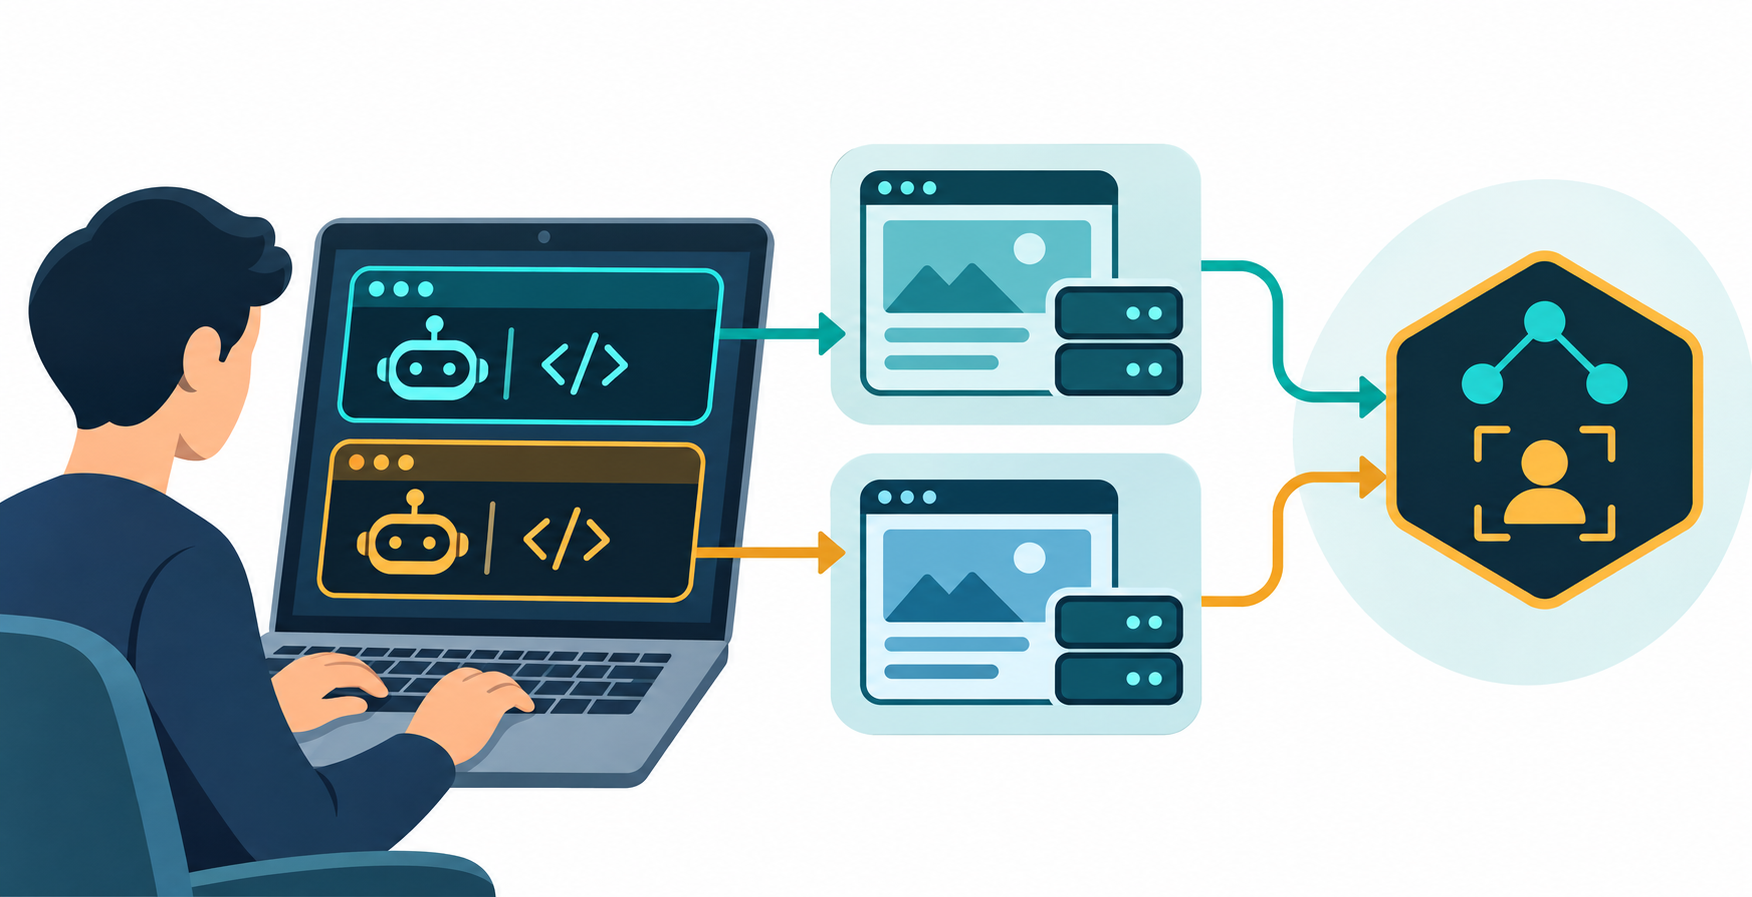
\includegraphics[width=0.54\linewidth]{assets/member-a-linking-concept.png}\\[-1mm]
{\scriptsize\emph{Concept only: one enrolled PC, two local agents, two partner sites, and one private correlator;
no experiment was run.}}
\vspace{1mm}

\noindent
\begin{minipage}[t]{0.485\linewidth}
\colorbox{navy}{\parbox{0.965\linewidth}{\color{white}\bfseries Mock input 1 --- Omen / Site 1}}
\fbox{\parbox{0.94\linewidth}{\scriptsize\ttfamily
run: a-sim-omen-001\\
agent: Omen; model: llama3.2:3b q4\\
website record: TLS/HTTP req-101\\
benchmark: 5 cases x 5 repeats\\
TTFC median: 0.42 s\\
evaluation: 30.8 tokens/s\\
content stored: no; machine label: withheld}}
\end{minipage}\hfill
\begin{minipage}[t]{0.485\linewidth}
\colorbox{amber}{\parbox{0.965\linewidth}{\color{white}\bfseries Mock input 2 --- Queen / Site 2}}
\fbox{\parbox{0.94\linewidth}{\scriptsize\ttfamily
run: a-sim-queen-001\\
agent: Queen; model: llama3.2:3b q4\\
website record: TLS/HTTP req-205\\
benchmark: 5 cases x 5 repeats\\
TTFC median: 0.44 s\\
evaluation: 30.5 tokens/s\\
content stored: no; machine label: withheld}}
\end{minipage}

\vspace{2mm}
\begin{multicols}{2}
\section*{Expected input and reaction}
The two harness signatures may differ. The linker therefore compares private session profiles instead of demanding
identical request hashes. Two illustrative relative differences are
\[
d_{\mathrm{TTFC}}=\frac{|0.42-0.44|}{0.42+0.44}=0.023,
\]
\[
d_{\mathrm{TPS}}=\frac{|30.8-30.5|}{30.8+30.5}=0.0049.
\]
Suppose a fitted model returns $p(\mathrm{same\ PC})=0.960$. With a pre-registered $\theta=0.950$, the expected
decision is \term{probably\_same\_pc}. The measurements, coefficients, score, and decision are illustrative. A
website alone cannot obtain local inference timing.

\section*{Expected tracker output}
\fbox{\parbox{0.92\linewidth}{\scriptsize\ttfamily
pair: omen-001 $\leftrightarrow$ queen-001\\
agent labels: Omen $\neq$ Queen\\
same-pc score: 0.960 (simulated)\\
threshold: 0.950\\
decision: probably\_same\_pc\\
evidence: compatible benchmark curves\\
warning: not human or serial identity}}

\section*{Tracker workflow}
\begin{enumerate}[leftmargin=*,nosep]
\item Each partner site records only its own direct request.
\item The loopback collector adds timing/count fields only in the consented testbed.
\item Repetitions become one session profile; Omen and Queen profiles become a symmetric pair.
\item Training labels are pseudonymous machine aliases, never hostnames or serial numbers.
\item Evaluation reports false matches and false non-matches on held-out PCs.
\end{enumerate}

\section*{Counterexample and required test}
If background load changes Queen's example throughput to $20.0$ tokens/s,
\[
d_{\mathrm{TPS}}=\frac{|30.8-20.0|}{30.8+20.0}=0.213.
\]
The score may fall below $0.950$, yielding \term{unknown}, not a forced non-match. Conversely, two identical PCs
may produce a false link. The final campaign must include idle/load, reboot, network-change, same-NAT, and
identical-hardware conditions. Until then, the simulated match is not a research result.

\section*{What is now feasible}
The repository can preview the fixed plan, collect timing-only Ollama data, aggregate profiles, train with
whole-machine holdout, score every cross-agent pair, and produce \term{same\_pc\_probability} plus a conservative
decision. It cannot create scientific evidence without several independently labelled PCs and an untouched test.
\end{multicols}

\vfill
\colorbox{pale}{\parbox{0.965\linewidth}{\small\textbf{Reproducibility note.} Raw benchmark records, profiles,
models, and scores stay in the gitignored \term{data/benchmarks} directory. The public repository contains only
code, tests, the fixed protocol, and this explicitly simulated walkthrough.}}
\end{document}
